\section{Inverse Problem for wide Field of View Imaging} \label{radio}
So far the simplified inverse problem has been introduced. Each antenna pair measures a Fourier Component of the sky brightness distribution. The distance between antenna pairs dictates what point is sampled in the UV plane. This leads to the measurement equation \eqref{radio:eq:2dft}. Calculating the true image $X$ is simply inverting the two dimensional Fourier Transform.

\begin{equation}\label{radio:eq:2dft}
V(u, v) = \int\int X(x, y) e^{2 \pi i (ux+vy)} dx dx
\end{equation}

\begin{wrapfigure}{r}{0.5\textwidth}
	\vspace{-15pt}
	\centering
	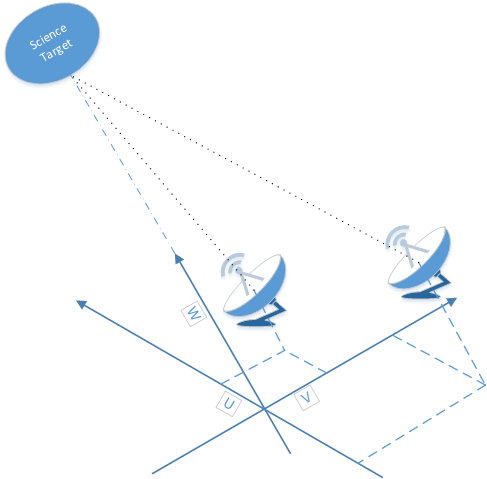
\includegraphics[width=0.9\linewidth]{./chapters/03.radio/uvw.png}
	\caption{U V and W coordinate space}
	\label{radio:uvw}
	\vspace{-10pt}
\end{wrapfigure}

In reality, each visibility has a third component $w$. It comes from the fact that the antennas are not on a flat plane but on the curved surface of the earth. Image \ref{radio:uvw} shows the three dimensional space. $w$ is the vector points from the phase center to the science target. For small Field of Views, the effect is negligible and the measurement equation \eqref{radio:eq:2dft} is a good approximation. The field of view is limited by the primary beam of the antennas. Primary beam widens with wavelength. So far, wide Field of View problems were encountered in low frequencies like LOFAR.


new instruments like SKA, ASKAP and Pathfinder are constructed with a wide Field of View in mind. The simple two dimensional Fourier Transform does not hold true anymore and we arrive at the wide Field of View measurement equation \eqref{radio:eq:ftSphere}.

\begin{equation}\label{radio:eq:ftSphere}
V(u, v, w) = \int\int \frac{X(x, y)}{\sqrt{1 - x^2 - y ^2}} e^{2 \pi i (ux+vy+ w\sqrt{1 - x^2 - y ^2})}dx dy
\end{equation}

Note that for small Field of View $1 - x^2 -y ^2 \ll 1$, and equation \eqref{radio:eq:ftSphere} can be approximated by the 2d Fourier Transform \eqref{radio:eq:2dft}. Two separate effects: $w$ Component for non coplanar baselines.

W-Projection \cite{cornwell2008noncoplanar}

A-Projection \cite{tasse2013applying}

All here to try to get back to the 2d fourier transform. 

"The field of view of a telescope is limited by the primary beams of the antennas. To map a region of sky where the emission is at a scale larger than the angular width of the primary beams, mosaicing needs to be done. This is discussed in the second part of this lecture."
Phase 

source \cite{lfraSchool}


Strength of compressed sensing is modelling these effects.

\subsection{Calibration}
A lot of effects, weather, noise, antenna temperature, drift.

Antenna based calibration, holds true for current interferometers but is not true for SKA. Possible switch to baseline based calibration.

\subsubsection{Self-Calibration}
?